% Original CSC302 teaching adaptation of Heather Macbeth, The Mechanics of Proof.
% Source: https://hrmacbeth.github.io/math2001/04_Proofs_with_Structure_II.html
% Source snapshot: e660f42b13ddcb6d12b52ba036d6bd071a0cfb9b (Lean 4.3).
% Mathematical statements are retained; exposition, exercises marked extension,
% and drawings are original. Lean fragments are demonstrations, not build-verified.
% CSC302 lecture slides adapted from Heather Macbeth, The Mechanics of Proof.
\documentclass[aspectratio=169,11pt]{beamer}
\usepackage[T1]{fontenc}
\usepackage{lmodern}
\usepackage{amsmath,amssymb,mathtools}
\usepackage{booktabs,array,listings,tikz}
\usetikzlibrary{arrows.meta,positioning,calc}
\definecolor{ProofNavy}{HTML}{18324F}
\definecolor{ProofTeal}{HTML}{007D82}
\definecolor{ProofPaper}{HTML}{F3F6F8}
\usetheme{default}
\setbeamercolor{normal text}{fg=ProofNavy,bg=white}
\setbeamercolor{structure}{fg=ProofTeal}
\setbeamercolor{frametitle}{fg=ProofNavy}
\setbeamercolor{block title}{fg=white,bg=ProofNavy}
\setbeamercolor{block body}{fg=ProofNavy,bg=ProofPaper}
\setbeamercolor{block title example}{fg=white,bg=ProofTeal}
\setbeamercolor{block body example}{fg=ProofNavy,bg=ProofPaper}
\setbeamerfont{frametitle}{size=\Large,series=\bfseries}
\setbeamertemplate{navigation symbols}{}
\setbeamertemplate{itemize item}{\small\textbullet}
\setbeamertemplate{footline}{%
  \leavevmode\hbox{%
  \begin{beamercolorbox}[wd=.86\paperwidth,ht=2.8ex,dp=1.2ex,leftskip=1.6em]{author in head/foot}%
    \scriptsize CSC302\quad\textbar\quad\insertshorttitle
  \end{beamercolorbox}%
  \begin{beamercolorbox}[wd=.14\paperwidth,ht=2.8ex,dp=1.2ex,rightskip=1.6em plus1fil]{date in head/foot}%
    \scriptsize\insertframenumber/\inserttotalframenumber
  \end{beamercolorbox}}}
\setbeamersize{text margin left=8mm,text margin right=8mm}
\lstdefinelanguage{Lean}{%
  morekeywords={example,theorem,lemma,def,by,calc,have,exact,apply,intro,intros,constructor,rcases,rfl,rw,ring,numbers,linarith,nlinarith,rel,extra,addarith,obtain,left,right,use,choose,dsimp,change,ext,fun,show,from,at,with,induction,case,decide,contradiction,push_neg,by_cases,by_contra,assumption,existsi,simp,simpa},
  sensitive=true,morecomment=[l]{--},morestring=[b]"}
\lstset{language=Lean,basicstyle=\ttfamily\small,keywordstyle=\color{ProofTeal}\bfseries,
  commentstyle=\color{gray},stringstyle=\color{ProofNavy},showstringspaces=false,
  columns=fullflexible,keepspaces=true,breaklines=true,frame=single,
  rulecolor=\color{ProofTeal!30},backgroundcolor=\color{ProofPaper},
  aboveskip=0.5em,belowskip=0.4em}
\newcommand{\N}{\mathbb{N}}
\newcommand{\Z}{\mathbb{Z}}
\newcommand{\Q}{\mathbb{Q}}
\newcommand{\R}{\mathbb{R}}
\newcommand{\coursechapter}[2]{%
  \title[Chapter #1: #2]{Chapter #1\\#2}%
  \subtitle{The Mechanics of Proof \textbar{} CSC302 lecture notes}%
  \author{Based on Heather Macbeth's textbook}%
  \date{}%
}
\newcommand{\sourcecredit}[1]{\par\vfill{\tiny Source: Heather Macbeth, \emph{The Mechanics of Proof}, #1.}}
\newcommand{\bookurl}{\url{https://hrmacbeth.github.io/math2001/}}
\hypersetup{colorlinks=true,urlcolor=ProofTeal,linkcolor=ProofNavy}

\coursechapter{4}{Proofs with structure, II}
\begin{document}
\begin{frame}\titlepage\end{frame}

\begin{frame}{What you should be able to do}
\begin{itemize}
\item Read nested quantifiers in the order in which they bind variables.
\item Prove both directions of an equivalence.
\item Separate the existence and uniqueness obligations in a claim.
\item Eliminate an impossible case and prove a negative statement.
\item Match each logical step to a small Lean tactic.
\end{itemize}
\begin{block}{Working convention}
Domains matter: $\N=\{0,1,2,\ldots\}$; $\Z$, $\Q$, and $\R$ have different possible witnesses. Lean snippets use the textbook's educational tactic environment.
\end{block}
\sourcecredit{Chapter 4, Sections 4.1--4.5}
\end{frame}

\section{4.1 For all and implication}
% Section 4.1, Examples 4.1.1, 4.1.4--4.1.6.
\begin{frame}{4.1: A universal statement is a reusable rule}
\begin{center}
\begin{tabular}{p{.25\textwidth}p{.30\textwidth}p{.30\textwidth}}
\toprule
Statement & To prove it & To use it\\\midrule
$\forall x\in A,\ P(x)$ & Fix an arbitrary $x\in A$. & Substitute a particular $t\in A$.\\[2mm]
$P\to Q$ & Assume $P$; prove $Q$. & Supply a proof of $P$ to obtain $Q$.\\\bottomrule
\end{tabular}
\end{center}
\[
\forall x\in\R,\quad x^2\le 2\ \longrightarrow\ x\le a
\]
This rule only supplies $t\le a$ after we establish $t^2\le 2$.
\begin{block}{Lean connection}
\texttt{intro x hx} introduces the object and its assumption.\quad
\texttt{exact h t ht} specializes a rule; \texttt{apply h} works backward.
\end{block}
\sourcecredit{Section 4.1}
\end{frame}

% Examples 4.1.1 and 4.1.5; original schematic graph.
\begin{frame}{A best lower bound: choosing versus fixing a variable}
\begin{columns}[T]
\begin{column}{.62\textwidth}
If $a\le x^2-2x$ for every real $x$, use $x=1$:
\[
a\le 1^2-2\cdot1=-1.
\]
Conversely, $-1$ is a lower bound because for an arbitrary $x\in\R$,
\[
x^2-2x=(x-1)^2-1\ge -1.
\]
Thus the largest lower bound is $-1$.
\end{column}
\begin{column}{.34\textwidth}
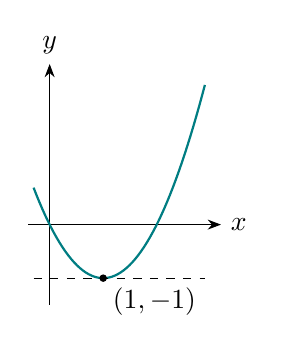
\begin{tikzpicture}[scale=.68,>=Stealth]
\draw[->] (-.4,0)--(3.2,0) node[right]{$x$};
\draw[->] (0,-1.5)--(0,3) node[above]{$y$};
\draw[thick,ProofTeal,domain=-.3:2.9,samples=60] plot (\x,{(\x-1)*(\x-1)-1});
\draw[dashed] (-.3,-1)--(2.9,-1);
\fill (1,-1) circle(2pt) node[below right]{$(1,-1)$};
\end{tikzpicture}
\end{column}
\end{columns}
\sourcecredit{Section 4.1, Examples 4.1.1 and 4.1.5}
\end{frame}

\begin{frame}[fragile]{Quantifiers determine the order of the proof}
Goal: $\exists b\in\R,\ \forall x\in\R,\ b\le x^2-2x$.
\begin{lstlisting}
-- Demonstration in the textbook's tactic environment.
example : Exists (fun b : Real =>
    forall x : Real, b <= x ^ 2 - 2 * x) := by
  use -1
  intro x
  calc
    -1 <= -1 + (x - 1) ^ 2 := by extra
    _ = x ^ 2 - 2 * x := by ring
\end{lstlisting}
The witness $b$ is chosen \emph{before} $x$ is introduced. It cannot depend on $x$.
\sourcecredit{Section 4.1, Example 4.1.5; ASCII teaching adaptation}
\end{frame}

% Examples 4.1.4 and 4.1.7.
\begin{frame}{A quantified hypothesis can prove uniqueness}
Suppose $a,b\in\R$ satisfy
\[
a^2\le2,\quad b^2\le2,\qquad
\forall y\in\R,\ y^2\le2\Rightarrow y\le a,
\]
\[
\forall y\in\R,\ y^2\le2\Rightarrow y\le b.
\]
\begin{enumerate}
\item Apply the rule for $b$ to $y=a$, using $a^2\le2$: obtain $a\le b$.
\item Apply the rule for $a$ to $y=b$, using $b^2\le2$: obtain $b\le a$.
\item Antisymmetry of $\le$ gives $a=b$.
\end{enumerate}
\begin{block}{Lean connection}
\texttt{apply le\_antisymm} produces the two inequalities. Each one is an application of a quantified implication.
\end{block}
\sourcecredit{Section 4.1, Example 4.1.4}
\end{frame}

\begin{frame}{``For all sufficiently large'' has a quantifier order}
For integers, this means
\[
\exists N\in\Z,\ \forall n\in\Z,\quad N\le n\Rightarrow P(n).
\]
For example, take $N=5$ to show $n^3\ge4n^2+7$ eventually.
For any integer $n\ge5$,
\[
n^3-4n^2=n^2(n-4)\ge n^2\ge25\ge7.
\]
The first inequality uses $n-4\ge1$ and $n^2\ge0$.
\begin{block}{What the proof supplies}
A single threshold works for every later input. It need not be the smallest possible threshold.
\end{block}
\sourcecredit{Section 4.1, Example 4.1.7}
\end{frame}

% Exercises 4.1.10, items 1, 3, 4.
\begin{frame}{4.1 Practice: identify the next object or assumption}
\begin{enumerate}
\item Let $a\in\Q$ and suppose $a\ge -3+4b-b^2$ for every $b\in\Q$. Prove $a\ge1$.
\item Prove $\exists n\in\N,\ \forall m\in\N,\ n\le m$.
\item Prove $\exists a\in\R,\ \forall b\in\R,\ \exists c\in\R,\ a+b<c$.
\end{enumerate}
\vspace{3mm}
For each proof, state which witnesses may depend on previously introduced variables.
\sourcecredit{Section 4.1, Exercises 4.1.10}
\end{frame}

\begin{frame}{4.1 Solution ideas}
\begin{enumerate}
\item Specialize the hypothesis at $b=2$:
\[
a\ge -3+4\cdot2-2^2=1.
\]
\item Choose $n=0$. Every natural number $m$ satisfies $0\le m$.
\item Choose $a=0$. After fixing an arbitrary $b$, choose $c=b+1$. Then $a+b=b<b+1=c$.
\end{enumerate}
\begin{block}{Dependency check}
In the third proof, $a$ is independent of $b$; $c$ is allowed to depend on $b$. Reversing quantifiers can change the problem.
\end{block}
\sourcecredit{Section 4.1, Exercises 4.1.10}
\end{frame}

\section{4.2 If and only if}
% Section 4.2, Example 4.2.1.
\begin{frame}[fragile]{4.2: An equivalence has two obligations}
\[
P\leftrightarrow Q\quad\text{means}\quad(P\to Q)\land(Q\to P).
\]
For $a\in\Q$,
\[
3a+1\le7\quad\Longleftrightarrow\quad a\le2.
\]
Forward: subtract $1$ and divide by positive $3$. Backward: multiply by positive $3$ and add $1$.
\begin{lstlisting}
-- Demonstration: each branch has its own assumption.
example (P Q : Prop) (forward : P -> Q)
    (backward : Q -> P) : Iff P Q := by
  constructor
  . exact forward
  . exact backward
\end{lstlisting}
\sourcecredit{Section 4.2, Example 4.2.1; adapted tactic demonstration}
\end{frame}

% Example 4.2.2.
\begin{frame}{Divisibility equivalence: the difficult direction needs an idea}
For $n\in\Z$, prove $8\mid5n\ \Longleftrightarrow\ 8\mid n$.
\begin{block}{Forward direction}
Write $5n=8a$ with $a\in\Z$. The identity $-3\cdot5+2\cdot8=1$ gives
\[
n=-3(5n)+16n=8(-3a+2n).
\]
The integer $-3a+2n$ is the divisibility witness.
\end{block}
\begin{block}{Backward direction}
If $n=8a$, then $5n=8(5a)$.
\end{block}
Do not cancel a factor in a divisibility statement without a reason; the coprimality of $5$ and $8$ is doing the work.
\sourcecredit{Section 4.2, Example 4.2.2}
\end{frame}

% Examples 4.2.5 and 4.2.7.
\begin{frame}{Solving an equation is an equivalence proof}
For a real number $x$,
\[
x^2+x-6=0\quad\Longleftrightarrow\quad x=-3\ \lor\ x=2.
\]
\begin{enumerate}
\item If the equation holds, then $(x+3)(x-2)=0$.
\item The zero-product rule gives $x+3=0$ or $x-2=0$.
\item These equations give the two candidate roots.
\item Conversely, substitution of either $-3$ or $2$ makes the original polynomial zero.
\end{enumerate}
\begin{block}{Lean connection}
\texttt{rw [mul\_eq\_zero] at h} turns a zero-product hypothesis into a disjunction. Use \texttt{obtain h1 | h2 := h} to handle its branches.
\end{block}
\sourcecredit{Section 4.2, Examples 4.2.5 and 4.2.7}
\end{frame}

% Exercises 4.2.10, items 1, 5.
\begin{frame}{4.2 Practice: prove the converse too}
\begin{enumerate}
\item For $x\in\R$, prove $2x-1=11\ \Longleftrightarrow\ x=6$.
\item For $k\in\N$, prove
\[
k^2\le6\quad\Longleftrightarrow\quad k=0\ \lor\ k=1\ \lor\ k=2.
\]
\item Explain why item 2 is false if $k\in\R$.
\end{enumerate}
Label the forward and backward directions before calculating.
\sourcecredit{Section 4.2, Exercises 4.2.10; domain check is an extension}
\end{frame}

\begin{frame}{4.2 Solution ideas}
\begin{enumerate}
\item Forward: $2x=12$, so $x=6$. Backward: $2\cdot6-1=11$.
\item If $k^2\le6$, then $k\ge3$ would imply $k^2\ge9$, a contradiction. Thus $0\le k\le2$, giving the three integer cases. Conversely, their squares are $0,1,4$, all at most $6$.
\item Over $\R$, $k=\tfrac12$ is a counterexample to the forward implication.
\end{enumerate}
\begin{block}{Proof habit}
A finite list follows from bounds only in a discrete domain. For an equivalence, checking the listed values proves only one direction.
\end{block}
\sourcecredit{Section 4.2, Exercises 4.2.10}
\end{frame}

\section{4.3 There exists a unique}
% Section 4.3, Example 4.3.1.
\begin{frame}{4.3: Existence plus uniqueness}
\[
\exists!x\in A,\ P(x)
\quad\Longleftrightarrow\quad
\exists x\in A,\ P(x)\land\forall y\in A,\bigl(P(y)\to y=x\bigr).
\]
To prove $\exists!a\in\R,\ 3a+1=7$:
\begin{enumerate}
\item \textbf{Choose:} $a=2$.
\item \textbf{Verify existence:} $3\cdot2+1=7$.
\item \textbf{Verify uniqueness:} for any $y$ with $3y+1=7$,
\[
y=\frac{(3y+1)-1}{3}=\frac{7-1}{3}=2.
\]
\end{enumerate}
\texttt{use 2}, then \texttt{constructor}, separates the two obligations in Lean.
\sourcecredit{Section 4.3, Example 4.3.1}
\end{frame}

% Example 4.3.3.
\begin{frame}{Use uniqueness by building a second candidate}
Let $x\in\Q$. Suppose exactly one rational $a$ satisfies $a^2=x$.
\begin{enumerate}
\item Existence supplies a rational $a$ with $a^2=x$.
\item The number $-a$ is another candidate: $(-a)^2=a^2=x$.
\item Uniqueness forces $-a=a$.
\item Therefore $2a=0$, so $a=0$ and $x=a^2=0$.
\end{enumerate}
\begin{block}{Why existence matters}
A rational number such as $-1$ has no rational square root. ``At most one'' would hold for it, but the conclusion $x=0$ would fail.
\end{block}
\sourcecredit{Section 4.3, Example 4.3.3}
\end{frame}

% Example 4.3.4. The argument is original but preserves the stated ranges.
\begin{frame}{A unique representative modulo 5}
Prove $\exists!r\in\Z$ such that $0\le r<5$ and $14\equiv r\pmod5$.
\begin{block}{Existence}
Take $r=4$: $14-4=5\cdot2$ and $0\le4<5$.
\end{block}
\begin{block}{Uniqueness}
If $0\le r<5$ and $14-r=5q$, then
\[
10\le14-r\le14,\qquad 2\le q<3.
\]
Since $q$ is an integer, $q=2$; hence $r=14-10=4$.
\end{block}
Without the interval restriction, $4,9,-1,\ldots$ all represent the same congruence class.
\sourcecredit{Section 4.3, Example 4.3.4}
\end{frame}

% Exercises 4.3.5, items 1 and 2.
\begin{frame}{4.3 Practice: do not stop after finding a witness}
\begin{enumerate}
\item Prove $\exists!x\in\Q,\ 4x-3=9$.
\item Prove $\exists!n\in\N,\ \forall a\in\N,\ n\le a$.
\end{enumerate}
For each item, write two separate sentences:
\begin{itemize}
\item The chosen object has the required property because \ldots
\item Every other object with the property equals it because \ldots
\end{itemize}
\sourcecredit{Section 4.3, Exercises 4.3.5}
\end{frame}

\begin{frame}{4.3 Solution ideas}
\begin{enumerate}
\item Choose $x=3$ and check $4\cdot3-3=9$. If $4y-3=9$, then $4y=12$ and $y=3$.
\item Choose $n=0$ and use $0\le a$ for each $a\in\N$. If $m\le a$ for every natural $a$, specialize at $a=0$. Then $m\le0$, and since $0\le m$, we obtain $m=0$.
\end{enumerate}
\begin{block}{Reusable pattern}
A universal property can identify a unique object by testing it at a strategically chosen input.
\end{block}
\sourcecredit{Section 4.3, Exercises 4.3.5}
\end{frame}

\section{4.4 Contradictory hypotheses}
% Section 4.4, Example 4.4.2.
\begin{frame}[fragile]{4.4: An impossible case imposes no further obligation}
If the assumptions give both $P$ and $\neg P$, they cannot all hold.
In logic, from this contradiction we may derive any target $Q$.
\begin{lstlisting}
-- Demonstration of the logical rule.
example (P Q : Prop) (hP : P) (hnP : Not P) : Q := by
  contradiction
\end{lstlisting}
For example, $t\in\Z$, $t<3$, and $t-1=6$ imply both $t=7$ and $7<3$.
\begin{block}{Interpretation}
The conditional theorem is valid because no input satisfies its assumptions. This is useful when eliminating a branch of a case split.
\end{block}
\sourcecredit{Section 4.4, Examples 4.4.1 and 4.4.2}
\end{frame}

% Example 4.4.1.
\begin{frame}{Rule out the wrong sign}
Let $x,y\in\R$, $x\ge0$, and $xy>0$. Prove $y>0$.
\begin{enumerate}
\item Split into $y\le0$ or $y>0$.
\item In the first case, multiplying by $x\ge0$ gives
\[
xy\le x\cdot0=0,
\]
contradicting $xy>0$.
\item In the second case, the desired conclusion is already available.
\end{enumerate}
\begin{block}{Where the hypothesis enters}
The condition $x\ge0$ justifies the direction of the inequality. Without it, $x=y=-1$ would be a counterexample.
\end{block}
\sourcecredit{Section 4.4, Example 4.4.1}
\end{frame}

% Example 4.4.3.
\begin{frame}{Residue cases can expose a contradiction}
For $n\in\Z$, suppose $n^2+n+1\equiv1\pmod3$.
\begin{center}
\begin{tabular}{ccc}
\toprule
$n\pmod3$ & $n^2+n+1\pmod3$ & Consequence\\\midrule
$0$ & $1$ & Allowed\\
$1$ & $0$ & Contradicts the assumption\\
$2$ & $1$ & Allowed\\\bottomrule
\end{tabular}
\end{center}
Thus $n\equiv0\pmod3$ or $n\equiv2\pmod3$.
\begin{block}{Lean connection}
\texttt{mod\_cases} creates the residue cases. The excluded case yields $0\equiv1\pmod3$; the textbook uses \texttt{numbers at H} on that numeric contradiction.
\end{block}
\sourcecredit{Section 4.4, Example 4.4.3}
\end{frame}

% Exercises 4.4.6, items 2 and 4.
\begin{frame}{4.4 Practice: eliminate impossible branches}
\begin{enumerate}
\item Let $x\in\Q$, $x^2=4$, and $x>1$. Prove $x=2$ by factoring and considering cases.
\item Let $n\in\Z$ and $n^2\equiv4\pmod5$. Prove
\[
n\equiv2\pmod5\quad\lor\quad n\equiv3\pmod5.
\]
\end{enumerate}
For each excluded case, state the contradictory pair of facts explicitly.
\sourcecredit{Section 4.4, Exercises 4.4.6}
\end{frame}

\begin{frame}{4.4 Solution ideas}
\begin{enumerate}
\item $(x+2)(x-2)=0$, so $x=-2$ or $x=2$. The first case gives $1<-2$, contradicting the numerical order. Therefore $x=2$.
\item Square the five possible residues:
\[
\begin{array}{c|ccccc}
n\pmod5&0&1&2&3&4\\\hline
n^2\pmod5&0&1&4&4&1
\end{array}
\]
Only residues $2$ and $3$ match the given square residue $4$.
\end{enumerate}
A case split is complete only when every branch is either solved or contradicted.
\sourcecredit{Section 4.4, Exercises 4.4.6}
\end{frame}

\section{4.5 Proof by contradiction}
% Section 4.5, Example 4.5.1.
\begin{frame}[fragile]{4.5: To prove a negation, assume its target}
The logical meaning of $\neg P$ is $P\to\mathrm{False}$.
To prove $\neg\forall x\in\R,\ x^2\ge x$, assume that universal claim and test $x=\tfrac12$.
\[
\left(\tfrac12\right)^2=\tfrac14<\tfrac12.
\]
\begin{lstlisting}
-- Demonstration in the textbook's tactic environment.
example : Not (forall x : Real, x ^ 2 >= x) := by
  intro h
  have H := h (1 / 2)
  numbers at H
\end{lstlisting}
The newly introduced assumption is discharged by the proof of the negation.
\sourcecredit{Section 4.5, Example 4.5.1}
\end{frame}

% Examples 4.5.2 and 4.5.8.
\begin{frame}{Why a number between consecutive multiples is not divisible}
For integers $a,b,q$, assume $bq<a<b(q+1)$. Then $b\nmid a$.
\begin{enumerate}
\item The interval is nonempty, so $bq<b(q+1)$ and hence $b>0$.
\item If $a=bk$ for some integer $k$, then
\[
bq<bk<b(q+1)\quad\Rightarrow\quad q<k<q+1.
\]
\item There is no integer strictly between consecutive integers.
\end{enumerate}
Example: $3\cdot4<13<3\cdot5$, so $3\nmid13$.
\begin{block}{Lean connection}
\texttt{intro h} assumes divisibility; \texttt{obtain} extracts its integer witness. The contradiction is an impossible bound on that witness.
\end{block}
\sourcecredit{Section 4.5, Examples 4.5.2 and 4.5.8}
\end{frame}

% Prime definition 4.1.8, composite test 4.5.7, prime_test 4.4.4.
\begin{frame}{A contradiction-based test for primality}
\begin{block}{Definition}
A natural number $p$ is prime when $p\ge2$ and every natural divisor of $p$ equals $1$ or $p$.
\end{block}
If $p=kl$ for $k,l\in\N$ with $k\ne1$ and $k\ne p$, then $p$ is not prime:
$k\mid p$, but neither allowed alternative holds.
\medskip
Equivalently, to prove $p$ prime, it suffices to show
\[
p\ge2,\qquad \forall m\in\N,\ 1<m<p\Rightarrow m\nmid p.
\]
A divisor of positive $p$ lies between $1$ and $p$. Eliminating the interior leaves exactly the two endpoints.
\sourcecredit{Sections 4.1, 4.4, 4.5; Examples 4.1.8, 4.4.4, 4.5.7}
\end{frame}

% Example 4.5.9. The proof compresses the original two-factor bound argument.
\begin{frame}{A smaller search interval for a prime test}
Let $p,T\in\N$. Assume
\[
p\ge2,\qquad p<T^2,\qquad
\forall m\in\N,\ 1<m<T\Rightarrow m\nmid p.
\]
Then $p$ is prime.
\begin{enumerate}
\item If $p$ were composite, write $p=ml$ with $1<m<p$.
\item Since $ml=p>m$, we have $l>1$.
\item If both $m\ge T$ and $l\ge T$, then $p=ml\ge T^2$, a contradiction.
\item One factor lies strictly between $1$ and $T$, contrary to the assumption.
\end{enumerate}
For $p=79$, use $T=9$ and check divisors $2,3,\ldots,8$.
\sourcecredit{Section 4.5, Example 4.5.9}
\end{frame}

% Example 4.5.4 and Exercise 4.5.10 item 9.
\begin{frame}{4.5 Practice: plan the contradiction before calculating}
\begin{enumerate}
\item Prove that no natural number $n$ satisfies $n^2=2$.
\item Use the improved prime test with $T=10$ to prove $97$ prime. For each $m=2,\ldots,9$, locate $97$ between consecutive multiples of $m$.
\end{enumerate}
For item 1, split the natural numbers at the boundary between $1$ and $2$.
\sourcecredit{Section 4.5, Example 4.5.4 and Exercises 4.5.10}
\end{frame}

\begin{frame}{4.5 Solution ideas}
\begin{enumerate}
\item If $n\le1$, then $n^2\le1<2$. If $n\ge2$, then $n^2\ge4>2$. Both cases contradict $n^2=2$.
\item We have $2\le97<10^2$. The lower quotients are:
\end{enumerate}
\begin{center}
\begin{tabular}{c|rrrrrrrr}
$m$&2&3&4&5&6&7&8&9\\\hline
$q$&48&32&24&19&16&13&12&10\\
$mq$&96&96&96&95&96&91&96&90
\end{tabular}
\end{center}
In every column, $mq<97<m(q+1)$, so $m\nmid97$. The improved prime test now applies.
\sourcecredit{Section 4.5, Example 4.5.4 and Exercises 4.5.10}
\end{frame}

\begin{frame}{Review: let the outermost logical symbol guide you}
\begin{center}
\begin{tabular}{lll}
\toprule
Goal & Mathematical action & Lean cue\\\midrule
$\forall x,\ P(x)$ & Fix an arbitrary $x$ & \texttt{intro x}\\
$P\to Q$ & Assume $P$ & \texttt{intro hP}\\
$P\leftrightarrow Q$ & Prove two implications & \texttt{constructor}\\
$\exists!x,\ P(x)$ & Witness, property, uniqueness & \texttt{use}, \texttt{constructor}\\
$\neg P$ & Assume $P$ and derive falsehood & \texttt{intro hP}\\
Any goal with $P,\neg P$ & Eliminate the impossible case & \texttt{contradiction}\\\bottomrule
\end{tabular}
\end{center}
Before leaving a proof, check domains, witness dependencies, both directions, and all cases.
\sourcecredit{Chapter 4, Sections 4.1--4.5}
\end{frame}

\begin{frame}{Sources and further work}
Heather Macbeth, \emph{The Mechanics of Proof}, Chapter 4.
\begin{itemize}
\item 4.1: universal quantification, implication, and eventual properties.
\item 4.2: equivalence and complete solution sets.
\item 4.3: existence and uniqueness.
\item 4.4--4.5: contradictions, nonexistence, and prime tests.
\end{itemize}
\medskip
\href{https://hrmacbeth.github.io/math2001/04_Proofs_with_Structure_II.html}{Read Chapter 4 and its remaining exercises.}
\medskip

These slides use original teaching prose and drawings. Example and exercise numbers in source comments identify the adaptation. Lean demonstrations use the textbook's educational tactics.
\end{frame}
\end{document}
